\documentclass[utf8]{ctexart}
\usepackage{graphicx}
\usepackage{amsmath,amssymb,amsthm}
\usepackage{geometry}
\usepackage{enumitem}
\usepackage{xcolor}
\usepackage{mdframed}
\usepackage{tikz}
\usepackage{booktabs,array}
\usepackage{needspace}
\usetikzlibrary{arrows.meta,positioning,calc}
\geometry{a4paper,margin=2.5cm}

\newtheoremstyle{mystyle}
  {8pt}{8pt}{\kaishu}{0pt}{\bfseries}{}{1em}{}
\theoremstyle{mystyle}
\newtheorem{theorem}{定理}
\newtheorem{lemma}{引理}

\title{\textbf{人工智能导论\quad 第一次作业}}
\date{\today}
\author{李子嘉 2024012325}

\begin{document}
\maketitle

\section*{题目1}
\textbf{证明：}

当终点 $T$ 即将从边缘集（frontier）中取出时，树搜索的边缘集中仍有
最优路径上的某个节点 $n^*$，其对应路径为该最优路径的前缀，因而
\[
  g(n^*)+h^*(n^*)=h^*(S).
\]
由于 $T$ 的 $f$ 值最小，且 $h(T)=0$，故
\[
  g(T)=f(T)\le f(n^*)=g(n^*)+h(n^*).
\]

\subsection*{（1）}
代入 $h(n^*)\le h^*(n^*)+C_1$，得到
\[
  g(T)\le g(n^*)+h^*(n^*)+C_1=h^*(S)+C_1.
\]

\subsection*{（2）}
由边代价非负可知 $g(n^*)\ge0$，又有 $C_2\ge1$，因此
\begin{align*}
  g(T)
  &\le g(n^*)+C_2h^*(n^*)\\
  &\le C_2\bigl(g(n^*)+h^*(n^*)\bigr)
   =C_2h^*(S).
\end{align*}

\Needspace{15\baselineskip}
\subsection*{（3）}
\textbf{若已扩展的节点不重新打开，则上述结论不一定成立。}
考虑下列有向图，边上数字为代价：
\begin{center}
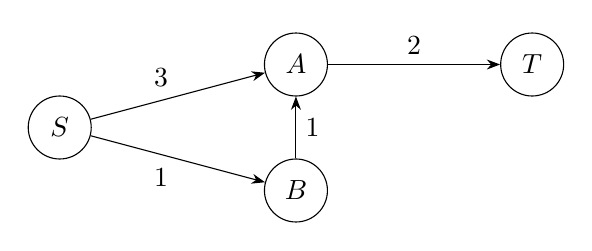
\begin{tikzpicture}[
  >=Stealth,
  vertex/.style={circle,draw,minimum size=8mm,inner sep=0pt},
  every edge/.style={draw,->},
  every edge quotes/.style={fill=white}
]
  \node[vertex] (S) at (0,0) {$S$};
  \node[vertex] (A) at (3,0.8) {$A$};
  \node[vertex] (B) at (3,-0.8) {$B$};
  \node[vertex] (T) at (6,0.8) {$T$};
  \draw[->] (S) -- node[above left] {$3$} (A);
  \draw[->] (S) -- node[below left] {$1$} (B);
  \draw[->] (B) -- node[right] {$1$} (A);
  \draw[->] (A) -- node[above] {$2$} (T);
\end{tikzpicture}
\end{center}
取启发函数如下：
\[
\begin{array}{c|cccc}
  n & S & A & B & T\\ \hline
  h^*(n) & 4 & 2 & 3 & 0\\
  h(n)   & 4 & 0 & 3 & 0
\end{array}
\]
各点均满足 $h(n)\le h^*(n)$，所以同时满足（1）中 $C_1=0$
和（2）中 $C_2=1$ 的条件。

扩展 $S$ 后，$f(A)=3$，$f(B)=4$，故先扩展 $A$，生成
$g(T)=5$ 的终点。随后扩展 $B$，虽发现了到 $A$ 的更短路径
$S\to B\to A$（代价为 $2$），但 $A$ 已关闭且不重新打开，
因此该路径不会继续传播到 $T$。最后取出 $T$，返回
\[
  g(T)=5>4=h^*(S),
\]
而最优路径为 $S\to B\to A\to T$，代价 $1+1+2=4$。
所以两个界都被违反。反例中的启发函数虽不高估，却不满足一致性，
因为 $h(B)=3>1+h(A)$。

\textbf{若发现更优路径时允许重新打开已关闭节点，}
则最优路径上仍能保留具有正确最优前缀代价的边缘节点，
（1）（2）的证明仍然适用。因此，不能仅凭采用图搜索就断言两个界必然失效。

% 后续题目继续使用 \section*{题目2} 等标题。
% 第二题按要求将本人学号题组的“答案正确”截图插入统一报告，无须另写逐步推导。
% 完成最终报告时，请自行调整文字，并按题面要求在末尾声明大模型辅助的方式和程度。

\end{document}
